\documentclass[10pt]{article}
\usepackage[ruled, linesnumbered]{algorithm2e}
\usepackage{Jan1, epsfig, subfigure, amssymb, multirow, algorithmic,amsmath}
\usepackage{latexsym,amssymb,epsfig,graphicx,subfigure,rotating,multirow,colortbl,xcolor,amsmath,algorithmic,booktabs,url}
\usepackage{accents}
\usepackage{subfig}
\textwidth 160mm
\textheight 225mm
\voffset 1mm
\oddsidemargin 1mm
\evensidemargin 1mm
\newtheorem{definition}{Definition}
\newtheorem{theorem}{Theorem}
\newtheorem{proposition}{Proposition}
\newtheorem{conjecture}{Conjecture}
\newtheorem{corollary}{Corollary}
\newtheorem{lemma}{Lemma}
\newtheorem{example}{Example}


\usepackage[english]{babel}
\usepackage{blindtext}

\usepackage{lipsum}

\newcommand\blfootnote[1]{%
  \begingroup
  \renewcommand\thefootnote{}\footnote{#1}%
  \addtocounter{footnote}{-1}%
  \endgroup
}






\title{ \hspace{3.2cm}
\includegraphics[scale=0.3]{./Fig/1.png} \newline \newline \newline  \LARGE{Comparison of QSS Solver's LIQSS2 solver with OpenModelica's DASSL solver}}

% \author{\large{Comparison of QSS Solver's LIQSS2 solver} \large{with OpenModelica's DASSL solver}}

% \date{\HUGE{Comparison of QSS Solver's LIQSS2 solver} \large{with OpenModelica's DASSL solver}}
\date{}


\renewcommand{\thefigure}{\arabic{section}.\arabic{figure}}
\renewcommand{\thetable}{\arabic{section}.\arabic{table}}
\begin{document}
\setcounter{page}{1}



\newcommand{\blokkie}{\hspace{.07cm}\Box\hspace{.07cm}}

%%%%% Set up the coloured tables %%%%%
\colorlet{tableheadcolor}{gray!25} % Table header colour = 25% gray
\colorlet{tablerowcolor}{gray!10} % Table row separator colour = 10% gray
\newcommand{\headcol}{\rowcolor{tableheadcolor}}
\newcommand{\rowcol}{\rowcolor{tablerowcolor}}

% The top-most line of a table
\newcommand{\topline}{\arrayrulecolor{black}\specialrule{0.1em}{\abovetopsep}{0pt}%
	\arrayrulecolor{tableheadcolor}\specialrule{\belowrulesep}{0pt}{0pt}%
	\arrayrulecolor{black}}

	% The top-most line of a table
\newcommand{\toplinee}{\arrayrulecolor{black}\specialrule{0.1em}{\abovetopsep}{0pt}%
	\arrayrulecolor{tablerowcolor}\specialrule{\belowrulesep}{0pt}{0pt}%
	\arrayrulecolor{black}}

% The line between the headings and the table body
\newcommand{\midline}{\arrayrulecolor{tableheadcolor}\specialrule{\aboverulesep}{0pt}{0pt}%
	\arrayrulecolor{black}\specialrule{\lightrulewidth}{0pt}{0pt}%
	\arrayrulecolor{white}\specialrule{\belowrulesep}{0pt}{0pt}%
	\arrayrulecolor{black}}

% A line for when the upper row is rowcolor and the next line is white
\newcommand{\midlinecbw}{\arrayrulecolor{tablerowcolor}\specialrule{\aboverulesep}{0pt}{0pt}%
	\arrayrulecolor{black}\specialrule{\lightrulewidth}{0pt}{0pt}%
 	\arrayrulecolor{white}\specialrule{\belowrulesep}{0pt}{0pt}%
	\arrayrulecolor{black}}

% A line with no black, to further separate a rowcolor row and a white row
\newcommand{\midlinecw}{\arrayrulecolor{tablerowcolor}\specialrule{\aboverulesep}{0pt}{0pt}%
	\arrayrulecolor{tablerowcolor}\specialrule{\lightrulewidth}{0pt}{0pt}%
	\arrayrulecolor{white}\specialrule{\belowrulesep}{0pt}{0pt}%
	\arrayrulecolor{black}}

% A line for when the upper row is white and the next line is rowcolor
\newcommand{\midlinewbc}{\arrayrulecolor{white}\specialrule{\aboverulesep}{0pt}{0pt}%
	\arrayrulecolor{black}\specialrule{\lightrulewidth}{0pt}{0pt}%
	\arrayrulecolor{tablerowcolor}\specialrule{\belowrulesep}{0pt}{0pt}%
	\arrayrulecolor{black}}

% sadfsdfsdf sdfsdfsdf
\newcommand{\midlinehr}{\arrayrulecolor{tablerowcolor}\specialrule{\aboverulesep}{0pt}{0pt}%
	\arrayrulecolor{black}\specialrule{\lightrulewidth}{0pt}{0pt}%
	\arrayrulecolor{tableheadcolor}\specialrule{\belowrulesep}{0pt}{0pt}%
	\arrayrulecolor{tablerowcolor}}


% A line for the bottom of the table, when the last row is white
\newcommand{\bottomline}{\arrayrulecolor{white}\specialrule{\aboverulesep}{0pt}{0pt}%
	\arrayrulecolor{black}\specialrule{\heavyrulewidth}{0pt}{\belowbottomsep}}%

% A line for the bottom of the table, when the last row is rowcolor
\newcommand{\bottomlinec}{\arrayrulecolor{tablerowcolor}\specialrule{\aboverulesep}{0pt}{0pt}%
	\arrayrulecolor{black}\specialrule{\heavyrulewidth}{0pt}{\belowbottomsep}}%

\newcommand{\bottomlinect}{\arrayrulecolor{tableheadcolor}\specialrule{\aboverulesep}{0pt}{0pt}%
	\arrayrulecolor{black}\specialrule{\heavyrulewidth}{0pt}{\belowbottomsep}}%
%%%%% Set up the coloured tables %%%%%



\maketitle



\pagestyle{myheadings}


\section{Introduction}

\blfootnote{Subject to NDA: Confidential \& Proprietary \copyright\ 2016 by LifeQ Global Limited. All Rights Reserved.}

The aim of this document is to compare QSS Solver's (stand-alone application) LIQSS2 solver~\cite{qss} with OpenModelica's DASSL solver. The actual results and the simulation times are of importance. We will provide insight into determining whether the LIQSS2 solver is adequate to use as LifeQ's solver for its VHM models.

A number of models will be compared. The models considered in this document are the standard models that are found in QSS Solver's test model suite. These models were specifically created by the authors of QSS Solver to showcase the savings in execution times as opposed to traditional ODE solvers.


\section{The solvers}

All the solvers used have been mentioned in \S1 of this document. These solvers include:
\begin{itemize}
 \item OpenModelica DASSL ({\sf OM\_DASSL})
 \item QSS Solver's LIQSS2 solver. ({\sf QSS\_LI2})
\end{itemize}

\section{Simulation details}

For each simulation run, the following will be specified:
\begin{itemize}
 \item duration of the simulation,
 \item some key state variables that will be investigated,
 \item the actual completion time of the simulation, and
 \item a conclusion of the obtained results.
\end{itemize}

For the DASSL solver in OpenModelica a tolerance of {\tt{1e-6}} is used and the number of intervals will be fixed at $10\,000$ for all simulations.

In QSS Solver and absolute tolerance of {\tt{1e-9}} and relative tolerance of {\tt{1e-6}} is used.

An Intel(R) Core(TM) i7-4710MQ CPU @ 2.50GHz computer containing 8 processors and 16GB RAM,
using operating system Linux Ubuntu 16.04 was used for the tests.



\section{Results}

The numerical results and related finding will be considered in this section. The computational times reported are in seconds and are the sum of the {\tt{user}} time and {\tt{sys}} time provided by the UNIX {\tt{time}} command, which is used in conjunction with the executable that is built for each model. The {\tt{user}} time is defined as the {\em total number of CPU-seconds that the process used directly (in user mode) in seconds}, while the {\tt{sys}} time is the {\em total number of CPU-seconds used by the system on behalf of the process (in kernel mode), in seconds}. The total time {\tt{user}}$+${\tt{sys}} indicates the total amount of actual CPU time a simulation uses.

\newpage

\subsection{Advection-Reaction model}

This model is the Method of Line discretization of an Advection-Reaction model, which leads to the set of ODEs:
\begin{eqnarray*}
 \dot{u}_i(t) &=& N\cdot(u_{i-1}(t) - u_i(t)) - \mu \cdot u_i(t) \cdot (u_i - \alpha)\cdot (u_i(t) - 1)
\end{eqnarray*}
with some initial equations specified.

This model was simulated for 1 second and for a total of 1\,000 state variables ($N= 1\,000$).

\begin{table}[htbp]
	\centering\footnotesize
		\begin{tabular}{ccp{8cm}}
    \topline	\headcol
    Solver&Sim time& Comments\\\midline
     \sf{OM\_DASSL}& 9.716&Correct simulation results obtained\\\rowcol
     \sf{QSS\_LI2}&0.492& Correct simulation results obtained \\\bottomlinec
    \end{tabular}
\caption{Simulation results of the Advection-Reaction model.}
\label{Tab2}
    \end{table}

    \begin{figure}[htbp]\centering
		\begin{tabular}{cc}

   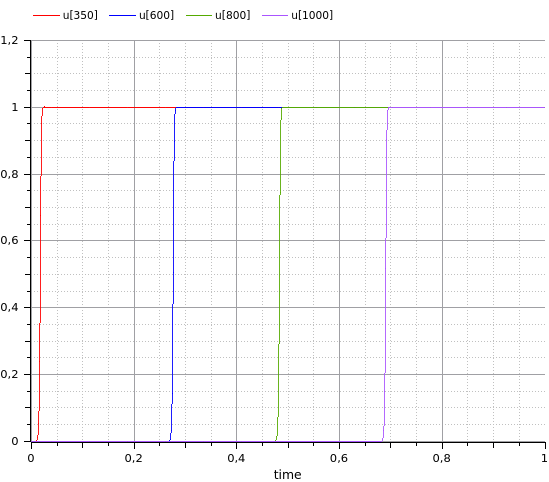
\includegraphics[scale=0.45]{./Fig/adv-om.png}&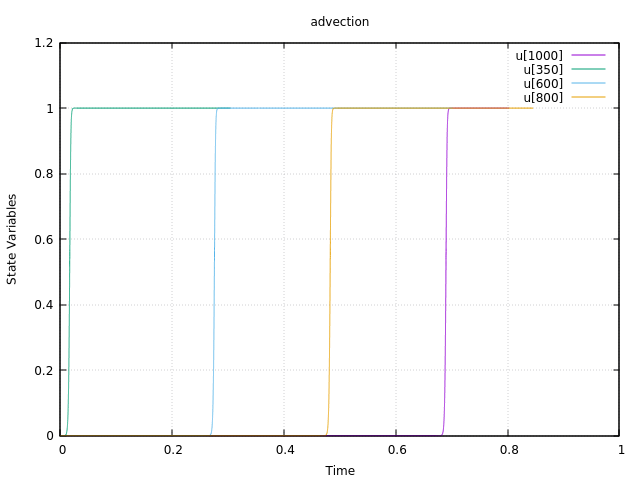
\includegraphics[scale=0.45]{./Fig/adv-liqss.png}\\(a) DASSL&(b) LIQSS2
    \end{tabular}
\vspace{-0.2cm}
\caption{Simulation results of the Advection-Reaction model.}\label{Fig1}
\end{figure}

\newpage

\subsection{Buck Converter}

A buck converter (step-down converter) is a DC-to-DC power converter which steps down voltage from its input to its output. The buck converter in this case consists of 4 branches.


This model was simulated for 0.01 seconds.

\begin{table}[htbp]
	\centering\footnotesize
		\begin{tabular}{ccp{8cm}}
    \topline	\headcol
    Solver&Sim time& Comments\\\midline
     \sf{OM\_DASSL}& 0.272&Correct simulation results obtained\\\rowcol
     \sf{QSS\_LI2}&0.016& Correct simulation results obtained \\\bottomlinec
    \end{tabular}
\caption{Simulation results of the Buck Converter.}
\label{Tab2}
    \end{table}

    \begin{figure}[htbp]\centering
		\begin{tabular}{cc}

   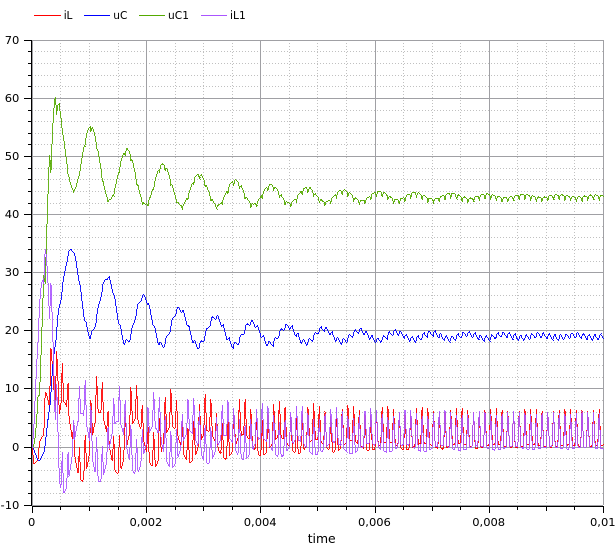
\includegraphics[scale=0.45]{./Fig/con-om.png}&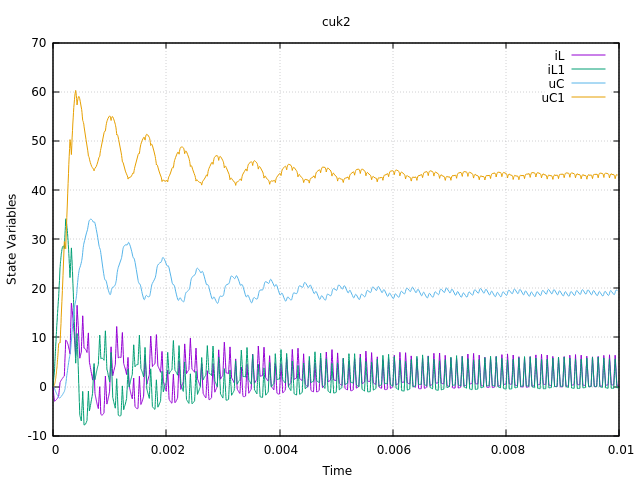
\includegraphics[scale=0.45]{./Fig/con-liqss.png}\\(a) DASSL&(b) LIQSS2
    \end{tabular}
\vspace{-0.2cm}
\caption{Simulation results of the Buck Converter.}\label{Fig1}
\end{figure}

\newpage

\subsection{Logical Inverter Chain}

This model is the represents a chain of $m$ logical inverters:
\begin{eqnarray*}
 \dot{\omega}_j(t) &=& U_{op} - \omega_j(t) - \Upsilon \cdot g(\omega_{j-1}(t), \omega_j(t))^2
\end{eqnarray*}
with $j =1,\ldots, m$ where
\begin{eqnarray*}
 g(u,v) = (\max(u - U_{th},0))^2 - (\max(u -v- U_{th},0))^2
\end{eqnarray*}


This model was simulated for 200 seconds. In this case we set $m =501$. Parameter values and initial values have also been set.

\begin{table}[htbp]
	\centering\footnotesize
		\begin{tabular}{ccp{8cm}}
    \topline	\headcol
    Solver&Sim time& Comments\\\midline
     \sf{OM\_DASSL}& 500.264&Correct simulation results obtained\\\rowcol
     \sf{QSS\_LI2}&0.160& Correct simulation results obtained \\\bottomlinec
    \end{tabular}
\caption{Simulation results of the Logical Inverter Chain.}
\label{Tab2}
    \end{table}

    \begin{figure}[htbp]\centering
		\begin{tabular}{cc}

   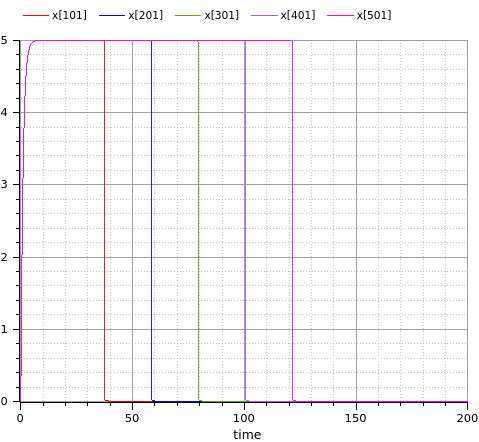
\includegraphics[scale=0.45]{./Fig/inv-om.png}&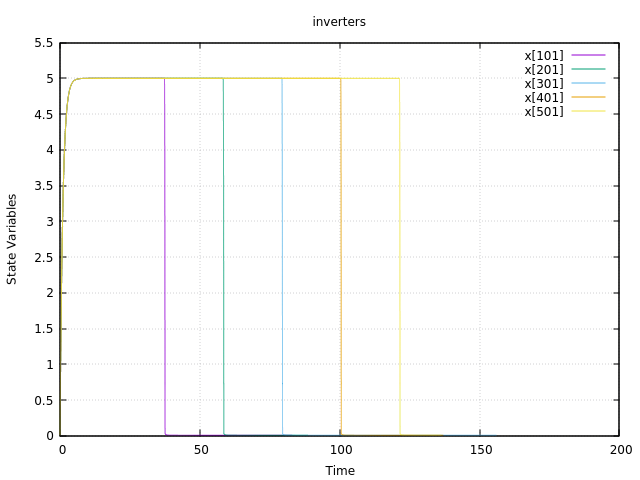
\includegraphics[scale=0.45]{./Fig/inv-liqss.png}\\(a) DASSL&(b) LIQSS2
    \end{tabular}
\vspace{-0.2cm}
\caption{Simulation results of the Logical Inverter Chain.}\label{Fig1}
\end{figure}

\newpage




\subsection{Bouncing Ball}

The bouncing ball is an example of a hybrid system, containing events and conditional expressions.

This model was simulated for 25 seconds.

\begin{table}[htbp]
	\centering\footnotesize
		\begin{tabular}{ccp{8cm}}
    \topline	\headcol
    Solver&Sim time& Comments\\\midline
     \sf{OM\_DASSL}& 0.020&Correct simulation results obtained\\\rowcol
     \sf{QSS\_LI2}&0.160& Correct simulation results obtained \\\bottomlinec
    \end{tabular}
\caption{Simulation results of the Bouncing Ball.}
\label{Tab2}
    \end{table}

    \begin{figure}[htbp]\centering
		\begin{tabular}{cc}

   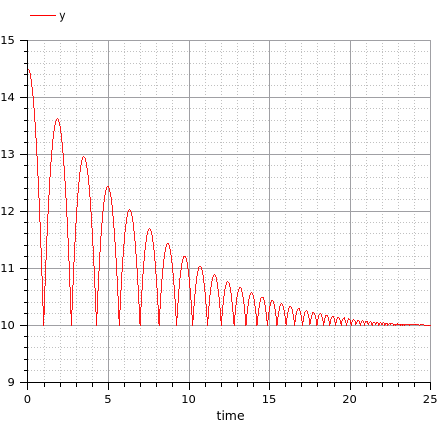
\includegraphics[scale=0.45]{./Fig/bal-om.png}&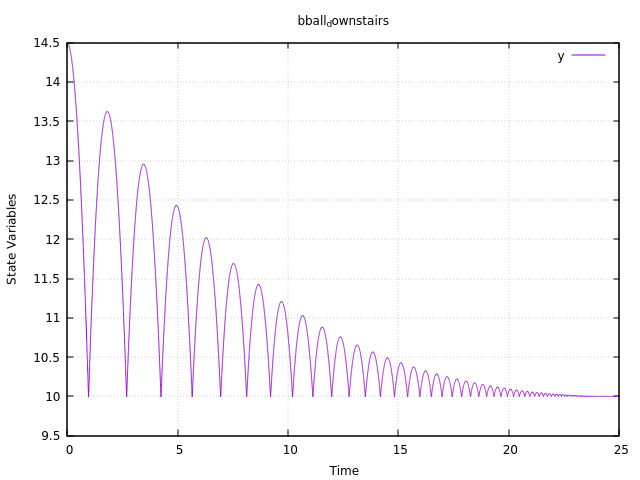
\includegraphics[scale=0.45]{./Fig/bal-liqss.png}\\(a) DASSL&(b) LIQSS2
    \end{tabular}
\vspace{-0.2cm}
\caption{Simulation results of the Bouncing Ball.}\label{Fig1}
\end{figure}

\newpage


\subsection{Rectifier}

I have no comments on this model. It is merely a model that is provided by QSS Solver.

This model was simulated for 2 seconds.

\begin{table}[htbp]
	\centering\footnotesize
		\begin{tabular}{ccp{8cm}}
    \topline	\headcol
    Solver&Sim time& Comments\\\midline
     \sf{OM\_DASSL}& 0.100&Correct simulation results obtained\\\rowcol
     \sf{QSS\_LI2}&1.548& Correct simulation results obtained \\\bottomlinec
    \end{tabular}
\caption{Simulation results of the Rectifier.}
\label{Tab2}
    \end{table}

    \begin{figure}[htbp]\centering
		\begin{tabular}{cc}

   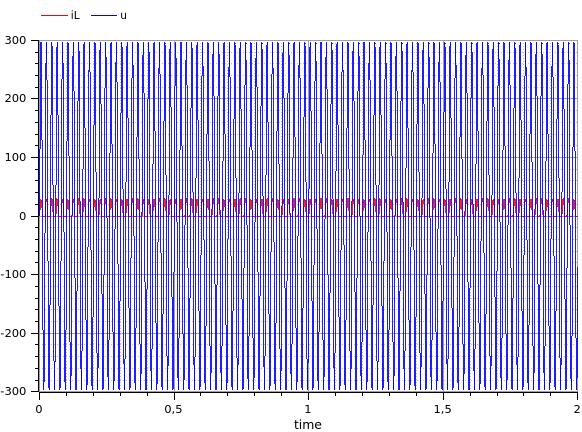
\includegraphics[scale=0.45]{./Fig/rec-om.png}&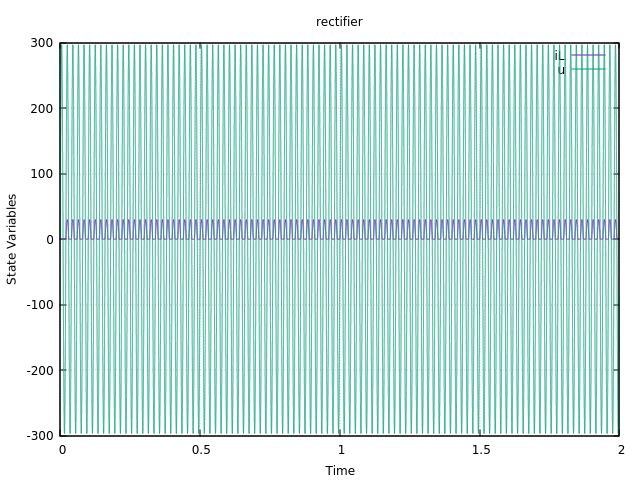
\includegraphics[scale=0.45]{./Fig/rec-liqss.png}\\(a) DASSL&(b) LIQSS2
    \end{tabular}
\vspace{-0.2cm}
\caption{Simulation results of the Rectifier.}\label{Fig1}
\end{figure}

\newpage



\section{Conclusion}

The first three models considered were stiff mathematical systems and the LIQSS2 solver was faster in all cases. The last two models were not stiff systems and DASSL was the faster solver in this case. So, this begs the question: ``{\em How dot he models compare when you have a both stiff components in the model as well as non-stuff ODE systems?}''

Lastly, I created a model that combines the advection-reaction model (a stiff mathematical system) with the bouncing ball (not a stiff mathematical system). From the results in the table below and some investigation both models take the largest portion of time simulating the stiff portion (the advection part). The bouncing ball part simulates quickly. The simulation run for this combination model was done for 5 seconds.


    \begin{table}[htbp]
	\centering\footnotesize
		\begin{tabular}{ccp{8cm}}
    \topline	\headcol
    Solver&Sim time& Comments\\\midline
     \sf{OM\_DASSL}& 10.206&Correct simulation results obtained\\\rowcol
     \sf{QSS\_LI2}&1.020& Correct simulation results obtained \\\bottomlinec
    \end{tabular}
\caption{Simulation results of the the combination of the advection model and the bouncing ball example.}
\label{Tab2}
    \end{table}


{\footnotesize
\begin{thebibliography}{10}

\bibitem{OMCompiler} {\sc OMCompiler}, 2016, {\em LifeQ OMCompiler submodule repository}, [Online], Cited 15\textsuperscript{th} March 2016, Available from {\url{https://bitbucket.org/antonpdv/omcompiler}}

\bibitem{OpenModelica} {\sc OpenModelica}, 2016, {\em Open Source Modelica Consortium}, [Online], Cited 15\textsuperscript{th} March 2016, Available from {\url{https://openmodelica.org/}}

\bibitem{DASSL}{\sc Petzold LR}, 1982, {\em A description of DASSL: A differential/algebraic system solver}, Technical Report, Applied Mathematics Division, Sandia National Laboratories, Livermore (CA).

\bibitem{qss}{\sc QSS Solver}, 2016, {\em Modeling and simulation tool for continuous and hybrid systems}, [Online], Cited 15\textsuperscript{th} March 2016, Available from {\url{https://sourceforge.net/projects/qssengine/}}



\end{thebibliography}}


\end{document}